\documentclass[letterpaper,twocolumn,10pt]{article}
\usepackage{usenix-2020-09}
    
\usepackage{tikz}
\usepackage{amsmath}
\usepackage{algpseudocode}
\usepackage{algorithm}

\begin{document}
%don't want date printed
\date{}

\title{\Large \bf OneRuleToFindThem: Efficient Automated Generation of Password Cracking Rules}

\author{
{\rm XXX}\\
AAA
\and
{\rm YYY}\\
BBB
\and
{\rm ZZZ}\\
CCC
}

\maketitle

\begin{abstract}
Password cracking tools such as Hashcat support the use of rules that transform
a dictionary of words, such as common English words and previously-cracked
passwords, into new candidate guesses for hashed passwords. Rules are necessary
to achieve high cracking ratios, however, they are difficult and time-consuming
to build by hand. We have developed an algorithm and implementation that
automatically finds successful rules via the combinatorial generation of rules
and empirical observation of how often each generated rule transforms a
dictionary word to a target password.

Our algorithm includes numerous performance and logical optimizations to avoid the
numerous pitfalls that would occur if a na\"ive brute-force technique were used.
In this paper, we explain our algorithm in detail and experimentally compare the
performance of its outputs to existing rule sets constructed via various
approaches ranging from fully-manual to fully-automated like our own.

We show that our approach is completely automated and achieves comparable
cracking performance to other top rule sets while also generating rules that
don't exist in other rule sets. This makes cracking attempts using our rules
mostly complementary to cracking attempts with other rule sets. Top performance is achieved by combining our generated rules with other rule sets.
\end{abstract}

\section{Introduction}

Although not the only form of authentication, the most common 
authentication for applications continues to be passwords. Properly implemented password
authentication and very strong passwords,
such as long passwords composed of random characters, is
generally effective. However, it is well-known that a significant proportion of
people elect to use passwords that combine a word with a few numbers or
special characters as required by the software. These passwords often
have predictable patterns and evolve in predictable ways over time as a user is
forced to change their password, often resulting in simple modifications
resulting in a new password with a high degree of similarity to the
original.\cite{hanamsagar2018leveraging} While this approach might make
passwords more amenable to memorization, it significantly weakens them in the
face of a password cracking attack.

A common approach to cracking passwords today is through the use of Hashcat,
utilizing the technique of hashing candidate passwords in a wordlist and
checking if the hash matches one found in list of password hashes. In order to avoid  a massive exhaustive
wordlist, Hashcat supports the use of `rules' which perform
transformations on a password. The resulting transformed passwords are then hashed and the same
checks are made. Examples include reverse (r), append character (\$X), and
replace (sXY, replace X with Y).\cite{hashcat}

% https://hashcat.net/wiki/doku.php?id=rule_based_attack
% https://hashcat.net/hashcat/

To produce the most guesses and therefore crack the most passwords, one must either have a large wordlist or a large number of rules (or both). However, because
most passwords are not generated randomly, some rules will be
(sometimes dramatically) more effective than others. Because each additional
rule in the list increases the time the cracking process takes to complete, an
attacker is incentivized to minimize the number of rules (and wordlist size) while maximizing the percent of hashes that are cracked. The attacker wishes to use on the most effective rules.

% TODO: better division, cracked/time

Many effective rules already exist and some are distributed with the
Hashcat software, such as the sizable `dive' list with about 99k rules. Various approaches have
been taken to produce these lists. Some creators manually curate rules, which
is a time-consuming process, while others have tried various algorithmic and
automated approaches. Often, existing rule sets are aggregated to various
degrees to produce a `super rule,' famously \textit{OneRuleToRuleThemAll} and
also some of the highly-effective `Pantagrule' lists of
rules.\cite{ortrta,pantagrule} The purpose of this paper is to detail a
novel fully-automated approach to rule generation, based on an iterative rule accumulation and scoring procedure. We compare the performance of our generated rule sets to existing publicly-available rules.

The rest of this paper is organized as follows. First, we review related work (Section~\ref{sec:related-work}. Next, we describe our algorithm in Section~\ref{sec:algorithm}. We do this in three parts. First, we show a simple brute-force procedure, then we explain optimizations we made to increase its effectiveness, followed by optimizations we made to increase its performance in terms of time and memory. Then we explain our experimental methodology (Section~\ref{sec:methodology}) followed by our results (Section~\ref{sec:results}), discussion (Section~\ref{sec:discussion}) and future work (Section~\ref{sec:future-work}).

% existence of aggregated rule sets (oneruletorulethemall, pantagrule)

% password change policies (regular intervals) might encourage people to make
% simple modifications to their existing password to create a new one; we want
% to find these by trying a trivial (primitive) modification one at a time until
% we hit a known password

% this approach has benefits because it can find unexpected combinations of
% primitive rules that might actually be somewhat common, however this approach
% also has the drawback of

\section{Related Work}
\label{sec:related-work}

Existing automated approaches to generating rules do exist. Several are based
on the PACK toolkit,\cite{PACK} a collection of tools designed for analyzing
password lists to detect masks, rules, character sets, and various other
password characteristics that can produce results designed to work with
Hashcat. The nsa-rules analysis by NSAKEY\cite{NSAKEY} and the rules it
generates take advantage of this toolkit as well as the more effective
Pantagrule rules.\cite{pantagrule}

Pantagrule rule lists were generated using PACK's Levenshtein reverse path
algorithm to produce rules which were then sorted by the frequenty at which
they were generated by PACK. This is similar to the approach NSAKEY took but
Pantagrule used a larger set of base passwords to generate rules, which
although initially public is now inaccessible. To further optimize the rules,
Pantagrule ran the top generated rules against the Pwned Passwords NTLM list
using the rockyou wordlist; ineffective rules were discarded. Several rule lists
are created from rules generated by various subsets of the seed data (top
passwords, random passwords, and a hybrid of the two).

A `one.rule' Pantagrule rule list builds upon the \textit{OneRuleToRuleThemAll}
rule list, which was created by concatenating and de-duping the top 25\% of
rules from various other rule lists.\cite{ortrta} `one.rule' appends top
performing Pantagrule hybrid rules to \textit{OneRule} and truncates the list
to the size of `dive.rule', a popular rule list distributed with hashcat.
\textit{OneRule} exceeds the performance of dive on its own, both in total \%
of passwords cracked and in cracking efficiency on the Lifeboat data dump.
Pantagrule's one.rule also compares favorably in total number of passwords
cracked against dive at the same total number of rules and against
\textit{OneRule} as a superset of its rules, however it is less efficient than
\textit{OneRule} as a consequence of containing significantly more total
passwords. Pantagrule suggests that their `one' peforms better than other known
lists the size of dive and they recommend it as a first list to try in a
cracking attempt.


% TODO: two ml approaches
In addition to traditional rule-based approaches to guessing passwords, some
techniques have been developed that attempt to avoid this entirely.
PassGAN\cite{hitaj2019passgan} is an approach that attempts to replace
rule-based password guessing with an approach based on deep learning and
generative adversarial networks (GANs). For PassGan a neural network was
trained to determine password characteristics and structures without making any
assumptions about these. Like our approach, PassGAN makes use of part of the
rockyou dataset and trains on it; they then tested their results against both
rockyou (with training data removed) and a leak of LinkedIn passwords. Their
results show that the PassGAN approach is able to match 34.6\% of passwords in
the rockyou dataset and 34.2\% in the LinkedIn dataset. While a typical
rule-based attack has the disadvantage of being able to exhaust guesses once
all rules have been applied to all initial passwords, PassGAN can generate
guesses effectively forever. So while PassGAN can in theory eventually guess
more passwords than any other approach, it needs to generate significantly more
passwords to do this as it can require up to 10x more guesses to reach the same
number of matched passwords as competitors. PassGAN also matches some passwords
not matched by any password rule in the rule sets they compared against.

Another approach\cite{pasquini2021improving} attempts to leverage
representation learning techniques to discover a representation of password
distributions. This technique models password representation through a GAN
instance and a Wasserstein Auto-Encoder (WAE) instance and two password guessing
frameworks are proposed; CPG and DPG. The model produced by this approach
improves on PassGAN against the rockyou test set, cracking 51.8\% of passwords
in the same number of guesses it took PassGAN to crack 34\%, $5 \times 10^{10}$.
Like PassGAN, the CPG and DPG frameworks guess some passwords that are not
cracked by other approaches and DPG allows a guessing attack to focus on unique
and otherwise ignored modalities of the target passwords.


% exact percent it says PassGAN cracked varies between PassGAN and pasquini
paper - both ~34% though

% - model the representation of passwords in the latent space of a GAN and of
%Wasserstein Auto-Encoders
%    - so semantically similar passwords are closer
%- using this representation, they can find passwords with strong locality and
%with weak locality
% PassGAN: TODO: WHERE:    - only considered passwords <= 10 characters
% TODO: pasquini - their GAN has a big improvement over PassGAN
% - locality is used to sample where to look next for password guessing

\section{Algorithm}
\label{sec:algorithm}

Our rule generator requires two inputs: a set of rule primitives that will be
combined to form complex rules, and a set of target passwords such as the
rockyou list. We implement an efficient version of what is essentially a
brute-force procedure. We first describe the brute-force procedure and then
describe our optimizations.


\subsection{Brute-force procedure}

Given each initial target password (e.g., from Rockyou), we apply every
primitive rule to the password to generate new passwords. For example, the
primitive Hashcat rule `r' (reverse) applied to the initial target password
`123456' results in password `654321.' We use a primitive rule set consisting
of elementary operations such as reverse (`r'), remove last character (`]'),
delete all `s' characters (`@s'), and so on, totaling nearly 400 primitive
rules. The selected password is subjected to every primitive, resulting in about
400 new passwords. For each resulting password (such as `654321'), we check if
it is one of our targets from our initial list of targets (e.g., Rockyou). If it
is, we boost the score of the rule that was applied. In the end, we have a list
of rules with scores indicating which rules were most successful.

After that initial step of applying rules to a single password, we proceed to
choose another password and apply all primitive rules to it, boosting the
scores of rules that transform the password to a known target password. We
choose the next password to try according to an ordering of the original target
list (e.g., Rockyou sorted by password `strength,' with weaker passwords chosen
earlier; details are given below).

Each password that is generated from applying primitive rules becomes a
potential candidate itself, unless it is already known from the initial target
set. For example, if the rule `r' is applied to `foobar,' producing `raboof,'
and `raboof' is not already known from the target set, it becomes a candidate
for selection. We record the history of rules that have already been applied, in
this case just `r.' When `raboof' is eventually selected as the next password to
try, each primitive rule is appended to its rule history, producing complex
rules `r ]' `r @s' and so on. If `]' applied to `raboof,' which produces
`raboo,' is a target, then we boost the score of the complex rule `r ].' We note
that the initial password `foobar' (pulled from Rockyou) was transformed to
`raboo' using complex rule `r ]' and `raboo' is a target (in this example,
though in reality it is not a member of Rockyou). Thus, our procedure has
discovered a successful rule that should be utilized in password cracking.

\begin{algorithm}\caption{Brute-force procedure, without optimizations}
\begin{algorithmic}[1]
\State $PrimitiveRules \gets $ fileContents(``primitives.rule'')
\State $Rules \gets PrimitiveRules$
\State $Targets \gets $ fileContents(``rockyou.txt'')
\ForAll {$p \in Targets$}
  \State $\mathrm{setRuleHistory}(p, \{\})$
\EndFor
\State $Candidates \gets Targets$
\State $Processed \gets \{\}$
\While{$|Candidates|\geq 0$}
  \State $p \gets \mathrm{chooseOne}(Candidates)$
  \State $Candidates \gets Candidates \setminus \{p\}$
  \State $Processed \gets \{p\} \cup Processed$
  \ForAll {$r \in PrimitiveRules$}
    \State $p' \gets \mathrm{applyRule}(p, r)$
    \State $H \gets \{r\}\cup\{\mathrm{append}(h, r)|h \in
\mathrm{ruleHistory}(p)\}$
    \State $\mathrm{setRuleHistory}(p', H)$
    \If {$p' \in Targets$}
      \ForAll {$h \in H$}
        \If {$h \in Rules$}
          \State $s \gets \mathrm{getScore}(h)$
          \State $\mathrm{setScore}(h,
s+\mathrm{strength}(p'))$
        \Else
          \State $\mathrm{setScore}(h, \mathrm{strength}(p'))$
          \State $Rules \gets \{h\}\cup Rules$
        \EndIf
      \EndFor
    \EndIf
    \If {$p' \notin Processed \cup Candidates$}
      \State $Candidates \gets \{p'\}\cup Candidates$
    \EndIf
  \EndFor
\EndWhile
\end{algorithmic}
\label{alg:brute-force}
\end{algorithm}

In summary, the brute-force procedure begins with an initial list of target
passwords and puts them into a candidate set, picks a single candidate password
at a time and applies all primitive rules, and boosts the scores of any rules
that ultimately produced a password found in the initial list of targets. Each
password generated from applying rules goes into the candidate set if it is not
already in there, and the sequence of primitive rules that generated it is
associated with the password.

Figure~\ref{fig:pwgen} shows an example of the combinatorial explosion of
candidates that results from the brute-force algorithm.

\begin{figure}[h!]
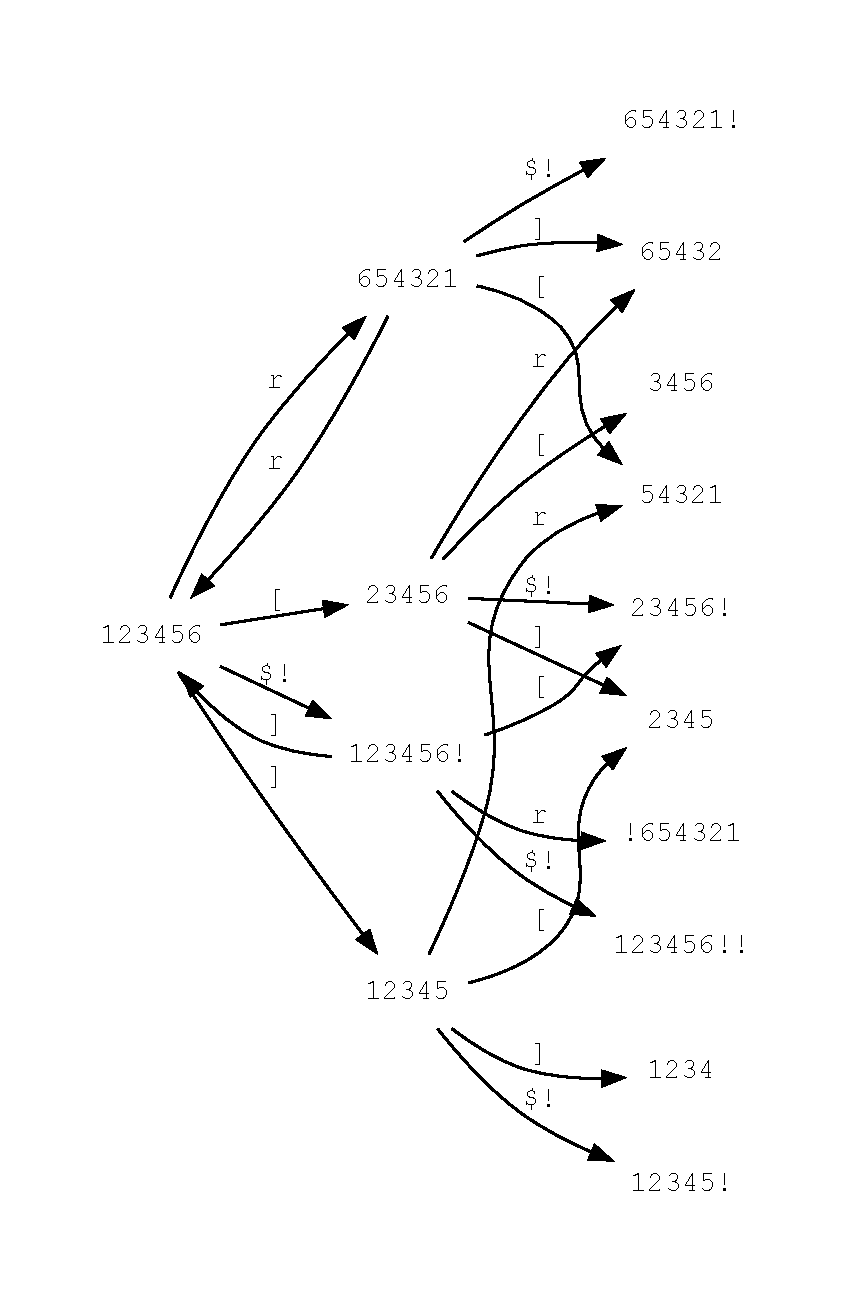
\includegraphics[width=\linewidth]{example-pw-rules.pdf}
\caption{Small example of the combinatorial explosion of passwords generated by
applying primitive rules. Note that some passwords may be reached by several
distinct rule histories, e.g., starting with password `123456,' the password
`54321' may be arrived at by applying complex rules `r [' or `] r,' or
even `\$! r [ [' (not shown in the graph).}
\label{fig:pwgen}
\end{figure}

\subsection{Optimizations for effectiveness}

The brute-force procedure suffers from significant drawbacks. Since it lacks
any criteria for checking rule validity and structure or for preferring to
examine some passwords before others, it is likely to generate worthless rules
and take a long time to do so.

\subsubsection{Hit a target only once}

The rockyou wordlist, which is our input to the algorithm, includes some very
basic words like `password' and even the single letter `a.' The brute-force
procedure will discover rules such as `] ] ] ] ] ] \$a' that will transform any
six-character password such as `gh\%@\_\$' into the password `a,' and the
procedure will boost the score of that rule. But that rule is hardly effective
for cracking password hashes. However, the procedure will boost that rule for
every six-character candidate because the rule will hit a target (namely, the
target `a'). When we allow this behavior, we see that the procedure yields
abundant variations of this logic (erasing characters from either end, then
adding a few to hit a small target), and they are not effective in experiments.

An easy way to prevent this behavior is to modify the `if' block starting on
line~17 in Algorithm~\ref{alg:brute-force} to what is shown in
Algorithm~\ref{alg:hit-target-once}.

\begin{algorithm}\caption{Hit a target only once}
\begin{algorithmic}
    \If {$p' \in Targets$}
      \ForAll {$h \in H$}
        \State \dots
      \EndFor
      \State $Targets \gets Targets \setminus \{p'\}$
    \EndIf
\end{algorithmic}
\label{alg:hit-target-once}
\end{algorithm}

\subsubsection{Ordering by password strength}

Because our algorithm applies all primitive rules to each candidate password,
we will produce hits faster if the candidate passwords we choose are those that
are the most likely to be transformed into a target password. Intuitively it
makes sense that the application of primitive rules to already very strong
passwords, such as long passwords consisting of random characters, would be less
effective than the application of rules to weaker passwords. In order to select
these weaker passwords earlier in our rule generation procedure we first
generate individual password strengths for a sample distribution of passwords.

For individual password strength we utilize a metric invented by Joseph Bonneau
called the `partial guessing metric,'\cite{bonneau2012statistical} which was
compared to other metrics and determined to be particularly effective.
Important properties of this metric are that it provides equal strength to all
passwords in a uniform distribution $\mathcal{U}_{N}$ % $\upsilon_{\mathit{N}}$
where each of $N$ events are equally likely and that it rates any event more
weakly than events less common in the distribution $\chi$.

This metric is developed with the assumption that the population-wide
distribution $\chi$ of passwords is completely known and addresses the issue of
estimating the strength of previously unseen passwords when a sample is used as
an approximation of $\chi$. For our approximation we use as a sample the
passwords in the rockyou dataset and the frequency at which they appear. We
produce a mapping of the passwords in our distribution to their strengths and
provide for estimating the strength of unseen passwords, allowing us to provide
each candidate encountered with a strength value.

With strength values known for all initial candidates and the ability to
determine the strength of new candidates we can create a priority queue where
high priority candidates are those with a low strength value. We select these
weaker candidates first, resulting in more hits of target passwords.

% TODO: also mention scoring rules w/ strength?

reducing strength for generated but unknown passwords


\subsubsection{Rule simplification}

The brute-force procedure appends each primitive rule to each rule in a
password's rule history on line~15. For example, if the password `password123'
was reached by iterative appending of primitive rules `\$1,' then `\$2,' then
`\$3,' the password will have rule history `\$1 \$2 \$3' (among others,
possibly). If `password123' is later selected as a candidate, each primitive
rule will be added to the end of that history and tested to see if it hits a
target. For example, `\$4' will be added and since `password1234' is a target,
each rule in the history (with `\$4' appended) will be boosted. Thus, the rule
`\$1 \$2 \$3 \$4' will be boosted.

We have identified numerous conditions in which complex rules (sequences of
primitive rules) are equivalent to a simpler rule. For example, the rule `\$1 ]
\$a' is equivalent to `\$a.' We also normalize rules by reordering some
sequences of primitives. For example, the rule `\^{}2 ] \^{}1' is equivalent to
`\^{}2 \^{}1 ]' (they both insert `12' at the front and remove the last
character). If we normalize all rules according to some common simplification
and sequencing logic, we can be sure to boost the normalized version of a rule
instead of boosting different variations and thus lowering the score of the
rule.

We have about 50 rule simplifications that are specified as regular
expressions. Table~\ref{tab:rule-simplification} shows the number of rules
generated originally (without simplification) and the number after simplifying,
for different lengths of rules. It is clear that exponential growth is still
present as the rule length increases. However, we benefit by ensuring we are
scoring the normalized rule rather than equivalent variations.

\begin{table}
\centering
\begin{tabular}{|l|l|l|l|}
\hline
Rule length & Original count & Simplified count & Ratio \\
\hline
1 & 313 & 313 & 1.0 \\
2 & 97,000 & 90538 & 0.93 \\
3 & 30,762,000 & 26,726,754 & 0.87 \\
4 & 296,735,000 & 255,805,952 & 0.86 \\
\hline
\end{tabular}
\caption{Impact of rule simplification. Rule length indicates number of
primitives in each complex rule; e.g., `r ] \$1' has length 3. Original count
specifies the number of rules generated with a certain length, without rule
simplification. Simplified count shows number of rules that remain after
rewriting some to a simpler form. Simpler forms will typically be repeats and
will be removed from the count.}
\label{tab:rule-simplification}
\end{table}

We modify the brute-force procedure with this optimization at line~15 by
first simplifying the new complex rule before adding it to the rule history.
This change is shown in Algorithm~\ref{alg:rule-simplification}.

\begin{algorithm}\caption{Rule simplification}
\begin{algorithmic}
    \State $H \gets \{r\}\cup\{\mathrm{simplify}(\mathrm{append}(h, r))|h \in%
\mathrm{ruleHistory}(p)\}$
\end{algorithmic}
\label{alg:rule-simplification}
\end{algorithm}

\subsubsection{No-op rule detection}

We also detect rules that accomplish nothing. For example, the rule `r r'
(reverse, then reverse again) will be boosted repeatedly since it essentially
does not transform a password at all. If the candidate password is already a
target, then the password generated by this rule is also a target (because it
is the same word), so `r r' will be boosted. In effect, the procedure will
yield abundant high-scoring rules that accomplish very little and will not be
effective for cracking hashes. These no-op rules are detected and eliminated as
shown in Algorithm~\ref{alg:eliminate-no-op}

\begin{algorithm}\caption{Eliminate no-op rules}
\begin{algorithmic}
    \State $H \gets H \setminus \{h|h\in H : \textrm{isNoOpRule}(h)\}$
\end{algorithmic}
\label{alg:eliminate-no-op}
\end{algorithm}

\subsubsection{Inventing primitive rules}

In order to facilitate generation of complex rules, we promote a complex rule
to the primitive rule set if the rule produces a target sufficiently often (we
experimentally chose this threshold to be 10 targets). For example, if the
primitive rule `\$3' is added to a rule history containing `\$1 \$2' and the
resulting complex rule `\$1 \$2 \$3' produces a target at least 10 times, then
`\$1 \$2 \$3' is added as a primitive. As a primitive, it will be added as a
single unit to other rules, e.g., it will be added to `\$1 \$2' as in this
example, yielding `\$1 \$2 \$1 \$2 \$3.' In our experimental results section,
we will show how many new primitive rules are invented.

\subsection{Optimizations for time and memory}

Other optimizations ensure our algorithm is time-efficient and uses limited
memory.

\subsubsection{Use of radix trees}

Because a password (potential new candidate) can be reached by many
combinations of primitive rules appled to a candidate, it is important for our
procedure to recognize which of these potential new candidates have already been
processed in order to avoid significant duplicate processing. The naive approach
of using a set very quickly becomes untenable with rapid growth in memory
consumption. To mitigate this, our procedure takes advantage of radix trees to
store unprocessed and processed passwords. The substring `password' in
`password123', `password!1', and `passwordxyz' will only be stored once. This
optimization dramatically slows down memory consumption as our process proceeds.

We make use of the same optimization to store our large number of generated
rules.

\subsubsection{Capping the candidate set}

The main growth of memory in the brute-force procedure is the result of
generating new password candidates. These candidates are saved to the queue and
processed according to the main loop starting on line~9 of
Algorithm~\ref{alg:brute-force}. In practice, we specify a maximum number of
cycles (i.e., how many times to repeat that loop), and we also choose a batch
of candidates at a time. We typically run for 1,000 cycles and choose 400
candidates at a time. We can compute the number of password candidates that
will ever be examined as the product of these two numbers (400,000). Whenever a
password is generated and it was not previously known, it is scored according
to its strength and added to a priority queue. Scores do not change after
candidates are added to the queue, so periodically (say, every 100 cycles), we
eliminate any members of the queue that are below the 400,000th position.

This technique allows us to cap the size of the candidate set. Doing so causes
the memory requirements to grow in terms of the size of the radix tree storing
the list of generated rules instead of the size of the candidate set. While the
brute-force procedure suffers from excessive growth of memory due to the
combinatorial nature of password generation, our more efficient variant reduces
the resident memory size, thus allowing a significantly longer run time, which
results in not only more rules but a better ordering of rules based on their
scores.

\section{Experimental Methodology}
\label{sec:methodology}

We chose to use the full rockyou wordlist containing about 14~million plaintext
passwords. This is our target set, and the original set of candidates. In order
to utilize our password strength metric, we require a target list that is
sorted by frequency of occurrence in real-world usage. rockyou is not sorted in
this way, but we can use the Pwned Hashes list, which includes frequencies.
Though Pwned Hashes contains hashes, not plaintext passwords, we can hash each
rockyou password and look up its frequency in the Pwned Hashes list, and order
rockyou by those frequencies.

We ran the algorithm for 1,000 cycles and 400 candidates per cycle, resulting
in 400,000 passwords being analyzed.

Our algorithm produces a list of rules. We remove logical duplicates using the `duperule' program~\cite{duprule}, which catches some duplicate rules that our rule simplifier misses. For example, it finds that `r ] \^{}n' (reverse, remove last, add `n' to front) is the same as `\$n r ]' (add `n' to end, reverse, remove last), so the latter rule is removed. With these deduplicated rules, we use Hashcat and the same rockyou wordlist to attempt to crack the most frequent 100~million Pwned Hashes. We record the percent cracked.

We compared performance of our rules against several other lists of rules,
including some that incorporate our own rules:

\begin{itemize}
\item An empty rule list, to see what percentage RockYou itself can crack.
\item Different sizes of our generated rules, ordered by rule score; e.g., top
10,000 rules, top 50,000, etc.
\item The `best64' and `dive' rules that come with the Hashcat distribution.
\item OneRuleToRuleThemAll with our generated rules appended, then trimmed to the size of the `dive' ruleset (99k rules), which we refer to as \textit{OneRuleToFindThem}.
\item One of Pantagrule's `one.rule' rule lists, equal in size to `dive'.
\item Pantagrule's top-performing and largest rules, pantagrule.private.v5.popular.
\item Pantagrule's rules pantagrule.private.v5.popular plus our generated rules, with duplicates removed from the combined set.
\end{itemize}

We also check the number of duplicate rules (according to the `duprule' program) that we share with other rules like OneRuleToRullThemAll, dive, and pantagrule.private.v5.popular.

\section{Results}
\label{sec:results}

A short list of the highest-scoring rules generated by our algorithm is shown
in Table~\ref{tab:top_rules}. These rules match our intuition about how people
typically modify an old password or dictionary word to make a new one.

While it is not the case that selecting only a `top-n' set of rules from our
generated rules produces a clear win against some common similarly-sized
rule sets like dive.rule (99k) or various Pantagrule rule sets, our results
clearly indicate that we are generating some strong rules that are not included
in these existing lists. In rarecoil's analysis of their Pantagrule rule sets
they compare `dive.rule' to a combination of OneRule and generated Pantagrule
rules (`one.rule', equal in size to dive) to demonstrate the utility of their
rules. At the time of its creation Pantagrule's `one.rule' performed better than
known lists equal in size to dive.

Our approach \textit{OneRuleToFindThem} compared to Pantagrule's highly
effective `one.rule' of
the same size demonstrates that we are XXXX
% TODO:
% more effective, making \textit{OneRuleToFindThem} the most effective rule
list of its size that we are aware of.
% This clearly demonstrates the efficacy of our approach to generating rules.
% OR?
% almost as effective, demonstrating the efficacy of our approach in nearly
reaching the most effective rule
% list of this size. Despite being marginally less effective, our approach uses
many different rules; this makes
% our approach to generating rules complementary to Pantagrule's and using both
during a cracking attempt should
% yield good results. Pantagrule notes that their approach only has a couple thousand rule overlap with \textit{OneRuleToRuleThemAll};
% this is true of our approach as well (XXXX).

While these comparisons demonstrate the effectiveness of our \textit{rules} in
comparison to the Pantagrule rule sets, they do not necessarily indicate the
effectiveness of our \textit{procedure} compared to the procedure used to
generate the Pantagrule rule sets. This is because while we used rockyou as our
wordlist, Pantagrule was developed with the use of a public but now
inaccessible wordlist. However, as Pantagrule describes their procedure we can
repeat their rule generation using the same wordlist we used, producing
effectively our own version of Pantagrule's `one.rule'. Comparing this to
\textit{OneRuleToFindThem} shows that the rulefile generated with our approach
XXXX %[cracked more passwords, %therefore indicating our procedure is more
effective | did not, :(]

\begin{table}
\centering
\begin{tabular}{|l|l|l|}
\hline
Rule & Score & Explanation \\
\hline
\$1 & 508,091 & Add `1' to end \\
T0 & 369,973 & Toggle case of first character \\
\$2 & 355,021 & Add `2' to end \\
t & 313,526 & Toggle case of all characters \\
\$7 & 290,926 & Add `7' to end \\
\$3 & 284,959 & Add `3' to end \\
] & 281,415 & Remove last character \\
\$1 \$2 & 273,308 & Add `12' to end \\
\$5 & 253,183 & Add `5' to end \\
\$4 & 246,386 & Add `4' to end \\
\$s & 239,729 & Add `s' to end \\
\$6 & 232,530 & Add `6' to end \\
\$1 \$2 \$3 & 229,973 & Add `123' to end \\
\hline
\end{tabular}
\caption{Top rules generated by our procedure. Scores represent relative
success at matching target passwords (an approximation of cracking success).}
\label{tab:top_rules}
\end{table}

\begin{figure}[h]
    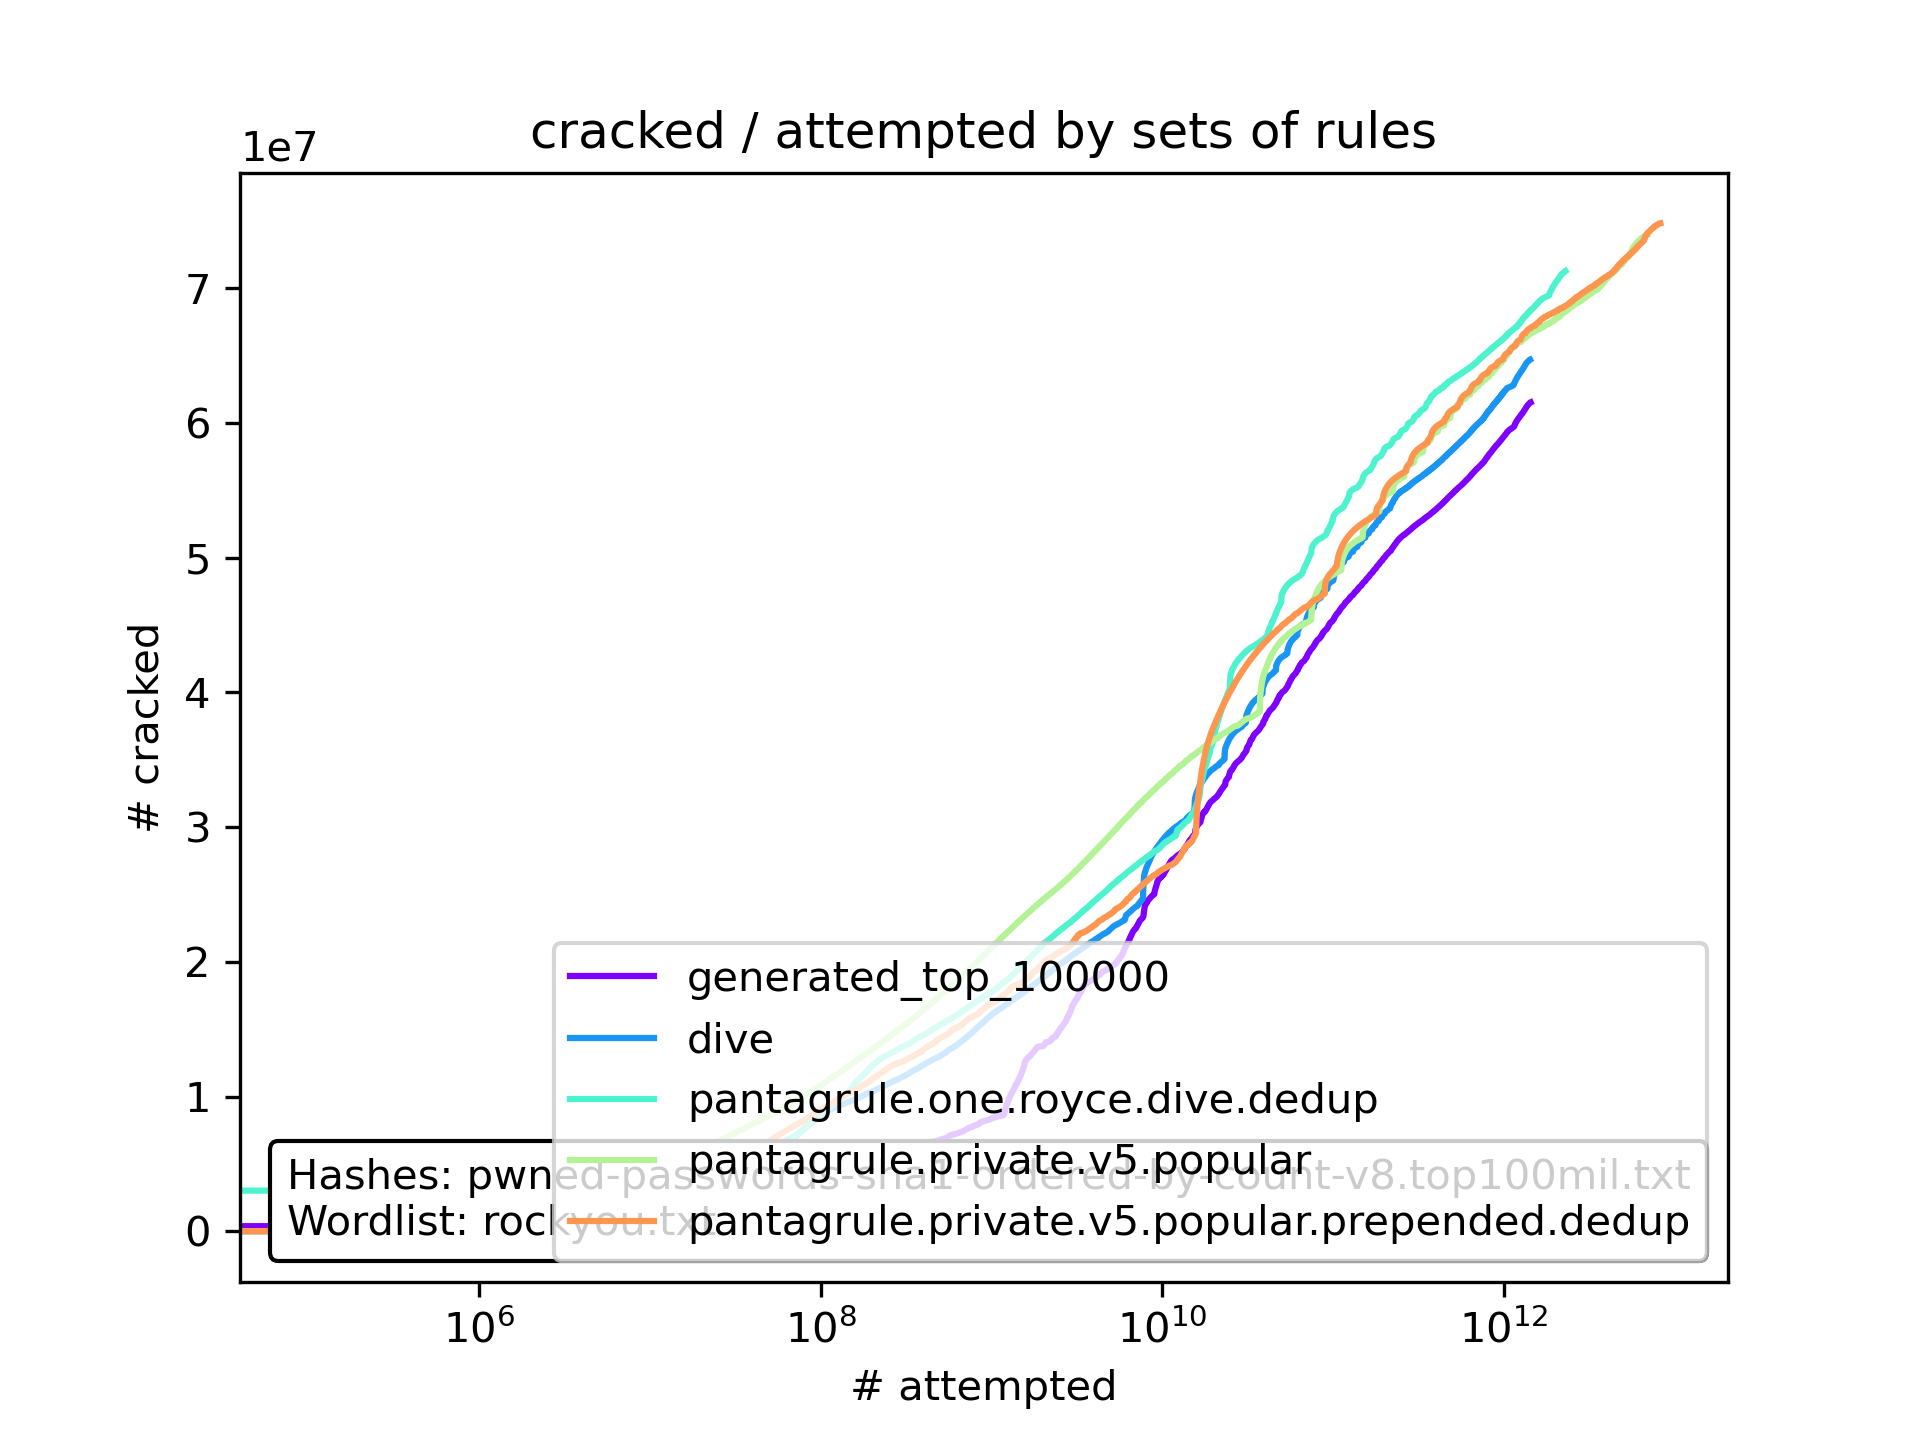
\includegraphics[width=\linewidth]
    {../cracked_attempted_plot_08318a9a-a503-11ed-9d73-005056c00001.png}
    \caption{NOT FINAL}
    \label{fig:cracked-attempted}
\end{figure}

\begin{table}
\centering
\begin{tabular}{|l|l|l|l|}
  \hline
  Rules & Count & Cracked & RPP \\
  \hline
  None (RockYou itself) & 0 & 6.33\% & 0 \\
  best64 & 64 & 24.99\% & 5 \\
  PACK top-64 & 64 & 24.57\% & X \\
  Ours top-10k & 10,000 & 34.97\% & 351 \\
  Ours top-50k & 50,000 & 55.24\% & 1025 \\
  ORTRTA & 51,998 & XYZ & XYZ \\
  dive & 99,092 & 64.71\% & 1701 \\
  ORTRTA+ours/trimmed & 99,092 & 69.66\% & 1568 \\
  PACK top-100k & 100,000 & 63.92\% & 1740 \\
  Ours top-100k & 100,000 & 58.28\% & 1930 \\
  Pantagrule-one+dive/dedup & 159,674 & 71.29\% & 2463 \\
  Ours top-300k & 300,000 & 65.70\% & 5063 \\
  Pantagrule-priv & 478,736 & 73.98\% & 7089 \\
  Pantagrule-priv+ours/dedup & 574,487 & 74.84\% & X \\
  \hline
\end{tabular}
\caption{Rules-per-password cracked metric (RPP) for various rule lists, ordered by size of the list. The formula for RPP is defined in the text.}
\label{tab:rpp}
\end{table}

\begin{table}
\centering
\begin{tabular}{|l|l|l|}
    \hline
    \% cracked & Best rules & RPP \\
    \hline
    $>5\%$ & No rules (RockYou itself) & 0 \\
    $>20\%$ & best64 & 5 \\
    $>60\%$ & ORTRTA+ours/trimmed & 1568 \\
    Max & Pantagrule-priv+ours/dedup & X \\
    \hline
\end{tabular}
\end{table}

Figure~\ref{fig:rule-count} shows that the number of complex rules grows per
cycle, but gradually levels off. Recall that a complex rule is created when it
has never been seen before and is able to transform a candidate password into a
target. Over time, fewer rules are generated that are both novel and
successful. Also recall that particularly successful rules are promoted to
primitives. The frequency of this occurrence also levels off, as shown in the
figure.

\begin{figure}[h]
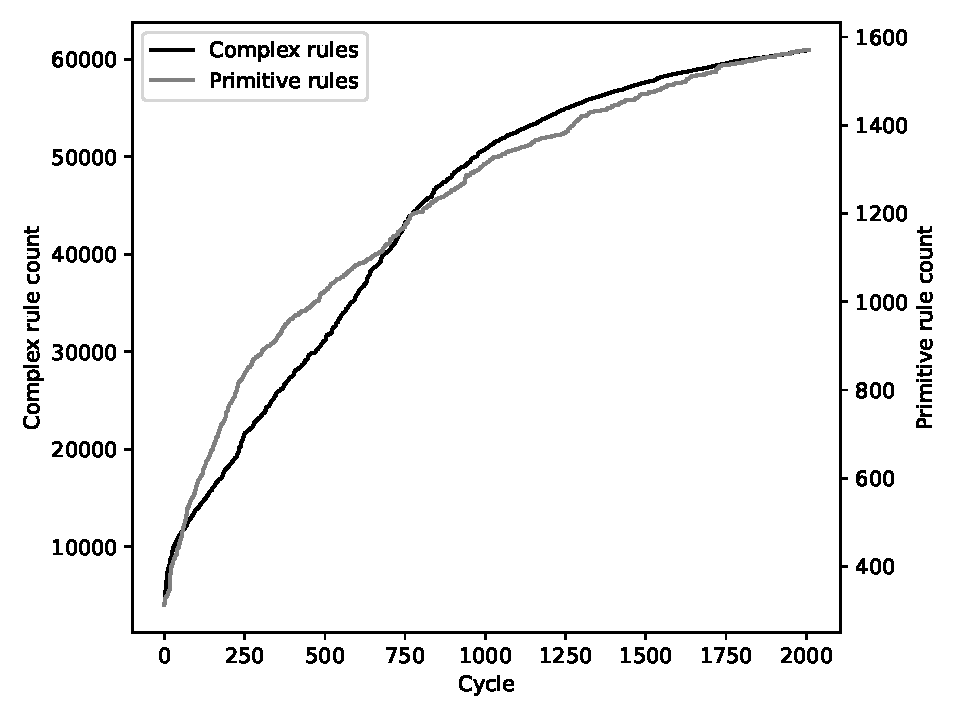
\includegraphics[width=\linewidth]
{analysis/passwords-analysis/stats-rules_composites_size.pdf}
\caption{Growth of complex and primitve rules over time (cycles). As targets
are hit, more complex rules are added. }
\label{fig:rule-count}
\end{figure}

The `duprule' program~\cite{duprule} eliminated 24,776 duplicate rules from our
generated set of 349,127 rules (7.1\%). Table~\ref{tab:dups} shows how many
deduplicated rules generated by our procedure are also found in various other
rule lists. The low `percent dup' values indicate that our generated rules do
not have much overlap with existing large rule sets. Thus, our techniques
compliment each other, and likely the best cracking performance may be obtained
by combining rule sets.

\begin{table}
\centering
\begin{tabular}{|l|l|l|l|}
    \hline
    Rules & Count & Duplicates & Pct. dup. \\
    \hline
    best64 & 64 & 47 & 73.4\% \\
    ORTRTA & 51,998 & 5,318 & 10.2\% \\
    dive & 99,092 & 3,712 & 3.7\% \\
    PACK-100k & 100,000 & 4,919 & 4.9\% \\
    Pantagrule private & 478,736 & 9,764 & 2.0\% \\
    \hline
\end{tabular}
\caption{Counts of rules that are found in both our generated rules and each
existing rule set. `ORTRTA' represents the rule set
`OneRuleToRuleThemAll'~\cite{ortrta}. `pantagrule private' refers to
Pantagrule's `pantagrule.private.v5.popular.rule'~\cite{pantagrule}. The `Count'
column indicates the count of rules in the rule set, the `Duplicates' column
indicates the count of rules in the rule set that match one of our generated
rules, and the `Pct. dup.' column is defined as the `Duplicates' column divided
by the `Count' column.}
\label{tab:dups}
\end{table}

In the early cycles of the algorithm, common passwords are selected from the
candidate set, and primitive rules are applied to them to generate new
passwords. We check if each generated password matches a target password, and
if so we call it a `hit.' Once a target password is hit, it is no longer
considered a target. Since many passwords in the RockYou list are simple
variations of other passwords in the list, we hit a lot of targets early but
fewer over time. This trend is shown Figure~\ref{fig:hitpct}. The decline in
hit percent appears to be exponential.

\begin{figure}[h]
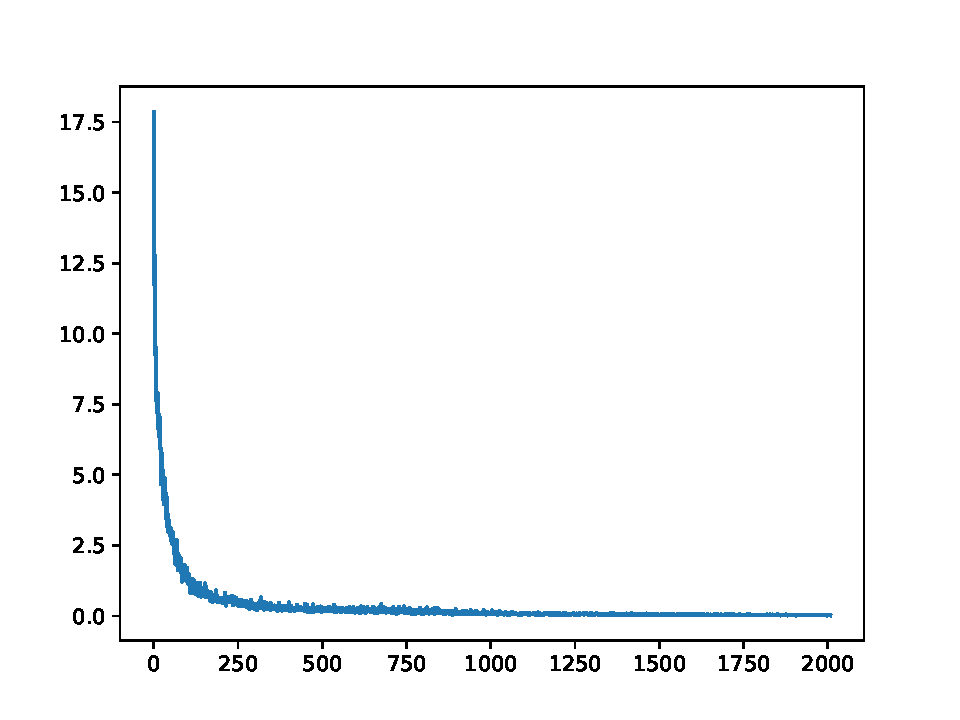
\includegraphics[width=\linewidth]
{analysis/passwords-analysis/stats-hitpct.pdf}
\caption{Percent of generated passwords that are target passwords (which we
call a `hit'), per cycle.}
\label{fig:hitpct}
\end{figure}

Figure~\ref{fig:seconds} shows the time required per cycle. As the number of
cycles increases, more rules have been generated and stored in the radix tree,
thus requiring more work to find and add rules.

\begin{figure}[h]
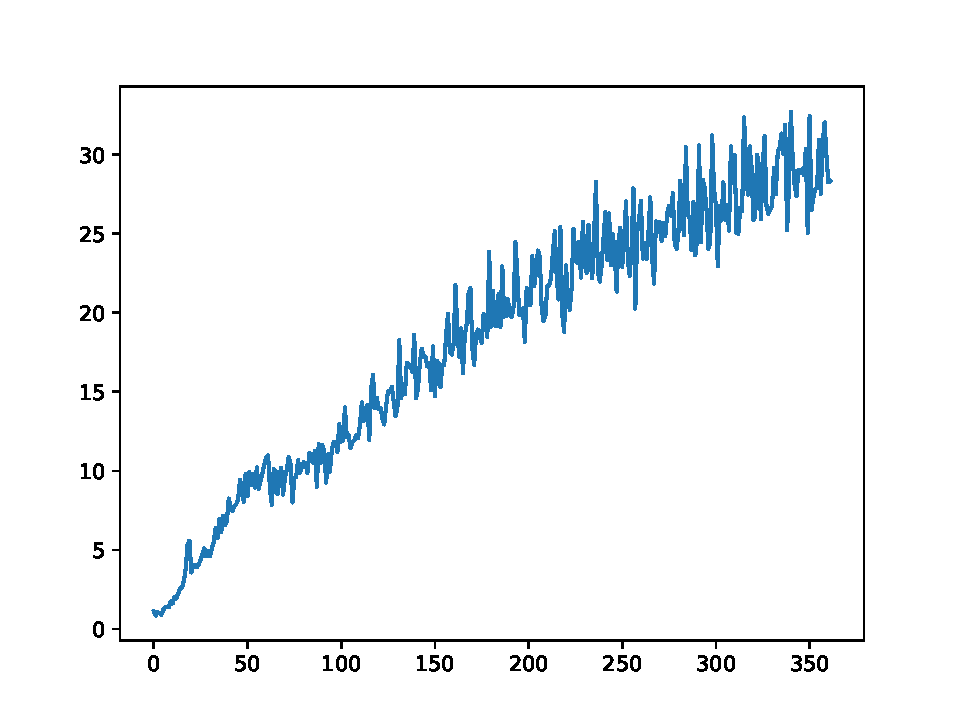
\includegraphics[width=\linewidth]
{analysis/passwords-analysis/stats-seconds.pdf}
\caption{Time per cycle. The spikes are due to the time required every 100
cycles to reduce the queue of candidates (a priority queue) to limit memory
growth.}
\label{fig:seconds}
\end{figure}

Figure~\ref{fig:memory} shows the growth of resident memory over time. The
growth is logarithmic and thus avoids the excessive memory use required by a
simple brute-force procedure. Note, however, that the memory usage grows past
60~GB, which is significant for consumer-grade computers. Memory usage can be
reduced by running the algorithm for fewer cycles (specified by a `max cycles'
parameter) and/or fewer password candidates chosen per cycle (also specified by
a parameter).

\begin{figure}[h]
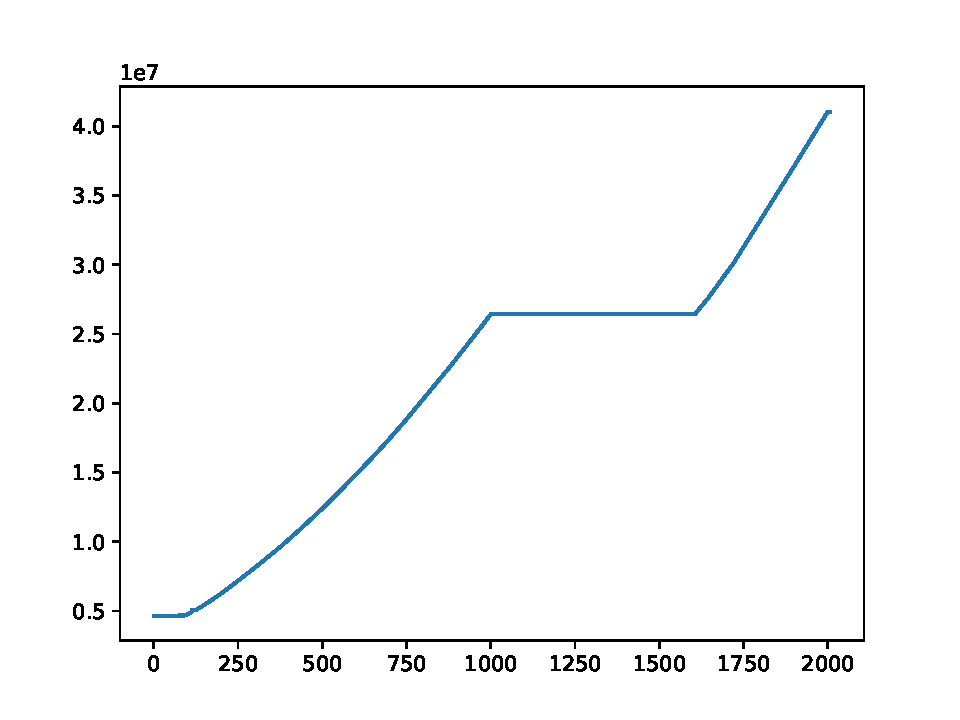
\includegraphics[width=\linewidth]
{analysis/passwords-analysis/stats-res_mem_size.pdf}
\caption{Resident memory per cycle. The growth is logarithmic due to the capped
candidate set size and the logarithmic growth of the radix tree storing
generated rules. The memory plot is not smooth because each 100 cycles memory
is reduced by trimming the candidate set size. However, the process keeps this
free memory space reserved for some time rather than releasing it back to the
operating system.}
\label{fig:memory}
\end{figure}

\section{Discussion}
\label{sec:discussion}

When we consider Figure~\ref{fig:rule-count} (rule
growth per cycle), Figure~\ref{fig:hitpct} (hit percent per cycle),
Figure~\ref{fig:seconds} (seconds per cycle), and Figure~\ref{fig:memory}
(memory per cycle) all together, we see that our algorithm expends a growing
amount of resources to generate a decreasing number of rules. The algorithm
produces diminishing returns. This is to be expected: the `easy' and most
successful rules are found early, while uncommon rules that hit password
targets that are infrequent (passwords that rarely appear in the Pwned Hash
set) are found rarely and only after extensive searching.

The same phenomenon can be observed in Table~\ref{tab:rpp}, which shows the
`rules-per-password cracked' (RPP) metric for various rule lists. This metric
estimates the number of rules required to crack a single password. With very
small lists of just the most effective rules, such as our XYZ or best64 from
Hashcat, one can crack a significant portion of hashes with minimal effort.
These are the `easy' hashes. The long-tail of rare passwords are much harder to
crack and require more work the greater their rarity.


\section{Future Work}
\label{sec:future-work}

explore use of word dictionaries

boost rule score only if rule produced a stronger password from a weaker one?

Interestingly, our research has also revealed that many existing lists of rules
include many rules that are functionally duplicates of each other, making the
cracking process unnecessarily longer. `duprule' or a similar program should
probably be run against most existing rule lists before using them in a cracking
attempt, and more research into making sure rule lists contain as few functional
duplicates as possible is certainly warranted.

\section*{Acknowledgments}

We wish to thank XYZ for his contributions to this project.

\section*{Availability}

Our code and results are available on GitHub at
\texttt{\href{https://github.com/REDACTED/REDACTED}
{github.com/REDACTED/REDACTED}}. We used various datasets
to generate our results:

\begin{itemize}
\item RockYou plaintext passwords:
\texttt{\href{https://github.com/zacheller/rockyou}
{github.com/ zacheller/rockyou}}
\item Pwned Passwords version 8, ordered by prevalence:
\texttt{\href{https://haveibeenpwned.com/Passwords}
{haveibeenpwned.com/Passwords}}
\item Pantagrule rules:
\texttt{\href{https://github.com/rarecoil/pantagrule}
{github.com/rarecoil/pantagrule}}
\item Common English words:
\texttt{\href{https://github.com/alex-pro-dev/english-words-by-frequency}
{github.com/alex-pro-dev/ english-words-by-frequency}}
\end{itemize}

Hashcat was used to measure the performance of rules:
\texttt{\href{https://github.com/hashcat/hashcat}{github.com/hashcat/hashcat}}.
We also used
`duprule,' a duplicate rule detector:
\texttt{\href{https://github.com/mhasbini/duprule}
{github.com/mhasbini/duprule}}.


%-------------------------------------------------------------------------------
\bibliographystyle{plain}
\bibliography{\jobname}

%%%%%%%%%%%%%%%%%%%%%%%%%%%%%%%%%%%%%%%%%%%%%%%%%%%%%%%%%%%%%%%%%%%%%%%%%%%%%%%%
\end{document}
%%%%%%%%%%%%%%%%%%%%%%%%%%%%%%%%%%%%%%%%%%%%%%%%%%%%%%%%%%%%%%%%%%%%%%%%%%%%%%%%

%%  LocalWords:  endnotes includegraphics fread ptr nobj noindent
%%  LocalWords:  pdflatex acks
